\documentclass{beamer}
\usetheme{default}
\usepackage[backend=bibtex]{biblatex}
\usepackage{dsfont}
\usepackage{graphicx}
\usepackage{epstopdf}
\usepackage{booktabs}
\usepackage{csquotes}
\bibliography{langonepresentationbib}


\title{Automated Protein Function Description}
\author{Meet Barot, PhD Student, Center for Data Science, NYU}

\begin{document}

\maketitle

\begin{frame}
    \frametitle{Intro}
    \begin{itemize}
        \item Machine learning for protein function prediction\pause
        \item Data: amino acid sequence, networks\pause
        \item deepNF\footfullcite{DeepNF}: integrating different types of edges in protein networks for a single organism\pause
        \item NetQuilt\footfullcite{NetQuilt}: integrating PPI networks of multiple organisms
    \end{itemize}
\end{frame}

\begin{frame}
\frametitle{Roadmap}
%High-throughput sequencing technologies have allowed us to amass millions of protein sequences from organisms throughout the tree of life.
\begin{enumerate}
    %\item Prior work in protein function prediction
    \item Protein function prediction $\rightarrow$ protein function description
    \item Motivation
    \item Model
    \item Evaluation metrics
    \item Results
\end{enumerate}
%Knowledge of protein function is necessary for understanding biological systems, but functional characterization is far outpaced by the discovery of new sequences from high-throughput sequencing technologies.
%Beyond the difficulty of assigning newly sequenced proteins to known functions, a more challenging issue is discovering novel protein functions.
%The space of possible functions becomes unlimited when considering designed proteins.
%Protein function prediction, as it is framed in the case of Gene Ontology term prediction, is a multilabel problem with a hierarchical label space.
%However, this framing is limiting. It does not provide guiding principles for discovering completely novel functions.
%Clustering-based approaches are not able to give much information about the new functional categories that they predict; they can only predict that a protein may belong to a category that has not been studied.
%In this work we propose a neural machine translation model in order to generate descriptions of protein functions in natural language.
%We provide quantitative results of our model in the zero-shot classification setting, scoring functional descriptions that the model has not seen before, as well as function descriptions for qualitative evaluation.
\end{frame}

%\begin{frame}
%\frametitle{Protein function prediction as it is}
%    \center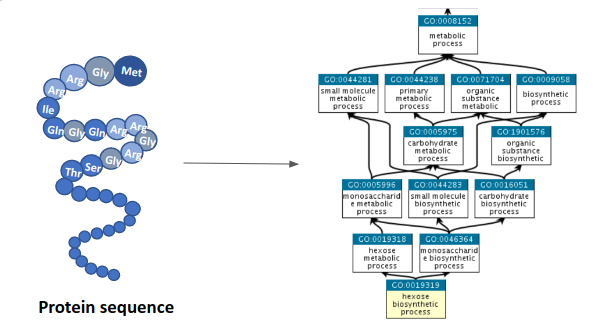
\includegraphics[height=0.4\textheight]{sequence_to_go_tree.png}
%    \begin{itemize}
%        \item Supervised function prediction methods rely on examples of known functions to predict only those known functions\pause
%        \item Their input data comes from sequence, structure, or protein-protein interaction networks \footfullcite{NetQuilt} to predict function
%    \end{itemize}
%\end{frame}


\begin{frame}
    \frametitle{Protein function prediction as it is}
    Supervised multilabel problem, where sequences are mapped to labels organized into a hierarchy, e.g. the Gene Ontology
    \center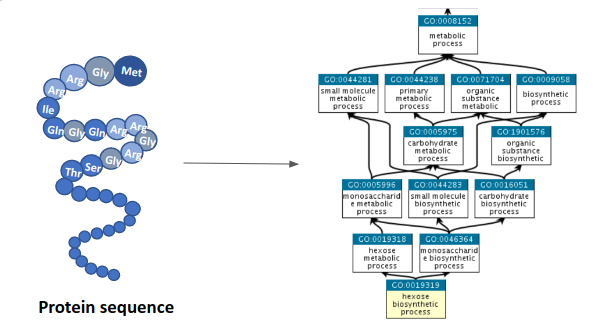
\includegraphics[height=0.4\textheight]{sequence_to_go_tree.png}
\end{frame}

\begin{frame}
    \frametitle{Protein function prediction as it \textbf{should be}}
    Given a set of proteins, describe their common function.
    \bigskip
    \begin{columns}
    \column{0.4\textwidth} 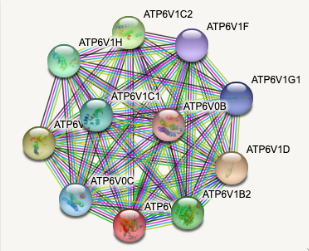
\includegraphics[height=0.4\textheight]{atpase_activity.png}
    \column{0.1\textwidth} \center $\rightarrow$
    \column{0.4\textwidth} ``Proton-transporting atpase activity, rotational mechanism."
    \end{columns}
\end{frame}

\begin{frame}
\frametitle{Motivation for protein function description}
    Why make a model that describes the common functions of a set of proteins in natural language?
\end{frame}

\begin{frame}
\frametitle{Motivation for protein function description}

    \begin{itemize}
        \item Why use sets of proteins?\pause
            \begin{itemize}
                \item A function description is our abstraction of the common property of a group of proteins. \pause
                \item We discover functions by understanding that a group of proteins do something in common.\pause
                %\item The \textit{data-generating process} here is: we observe a group of proteins, and we describe them with language to encapsulate what they do in common.
            \end{itemize}
        \item Why use natural language?\pause
            \begin{itemize}
                \item We can avoid having our predictions be limited to a pre-defined set of functions\pause
                \item With language, the model can compose new functions out of the same pieces that we use to explain the world to each other.\pause
            \end{itemize}
    \end{itemize}
    To discover new categories of protein function with info to guide experimental design to test for them, we need a model that generates functional descriptions.
\end{frame}

%\begin{frame}
%\frametitle{Current methods for function discovery}
%\begin{itemize}
%    \item Many methods exist for function prediction, but most do not consider the problem of discovering novel functions.\pause
%    \item Clustering-based methods are not able to give much information about the new functional categories that they predict\pause
%    \item DeepGOZero \footfullcite{DeepGOZero} predicts for terms not included in the training set, but this is limited to terms with ontological relations with known terms.
%\end{itemize}

%Clustering-based approaches are not able to give much information about the new functional categories that they predict.
%They can only predict that a protein may belong to a category that has not been studied.
%One could compute average distances to clusters that contain known proteins, but beyond this, there is no testable hypothesis that the model can give about their function.

%Zero-shot learning approaches attempt to address the unseen class problem as well, mostly by creating continuous embeddings of the labels and predicting a mapping from the input to real-valued vectors in that learned label space \cite{CLIP}.
%Similar to clustering-based approaches, not much information about the unseen class is gained besides its distance from existing categories and its direction in the abstract label space.
%DeepGOZero \cite{DeepGOZero} is a method that uses ontology axioms to predict for classes with no examples in the training set.
%However, the classes that are able to be predicted must be defined with ontological relations to seen classes.
%This constraint both restricts the possible novel functions that can be discovered and may not give sufficient information to design an experiment to test for the novel function.
%Among the few zero-shot approaches proposed for function prediction, none are able to describe the novel functions discovered in natural language.

%\end{frame}

\begin{frame}
\frametitle{Proposed model}
\begin{figure}
    \centering
    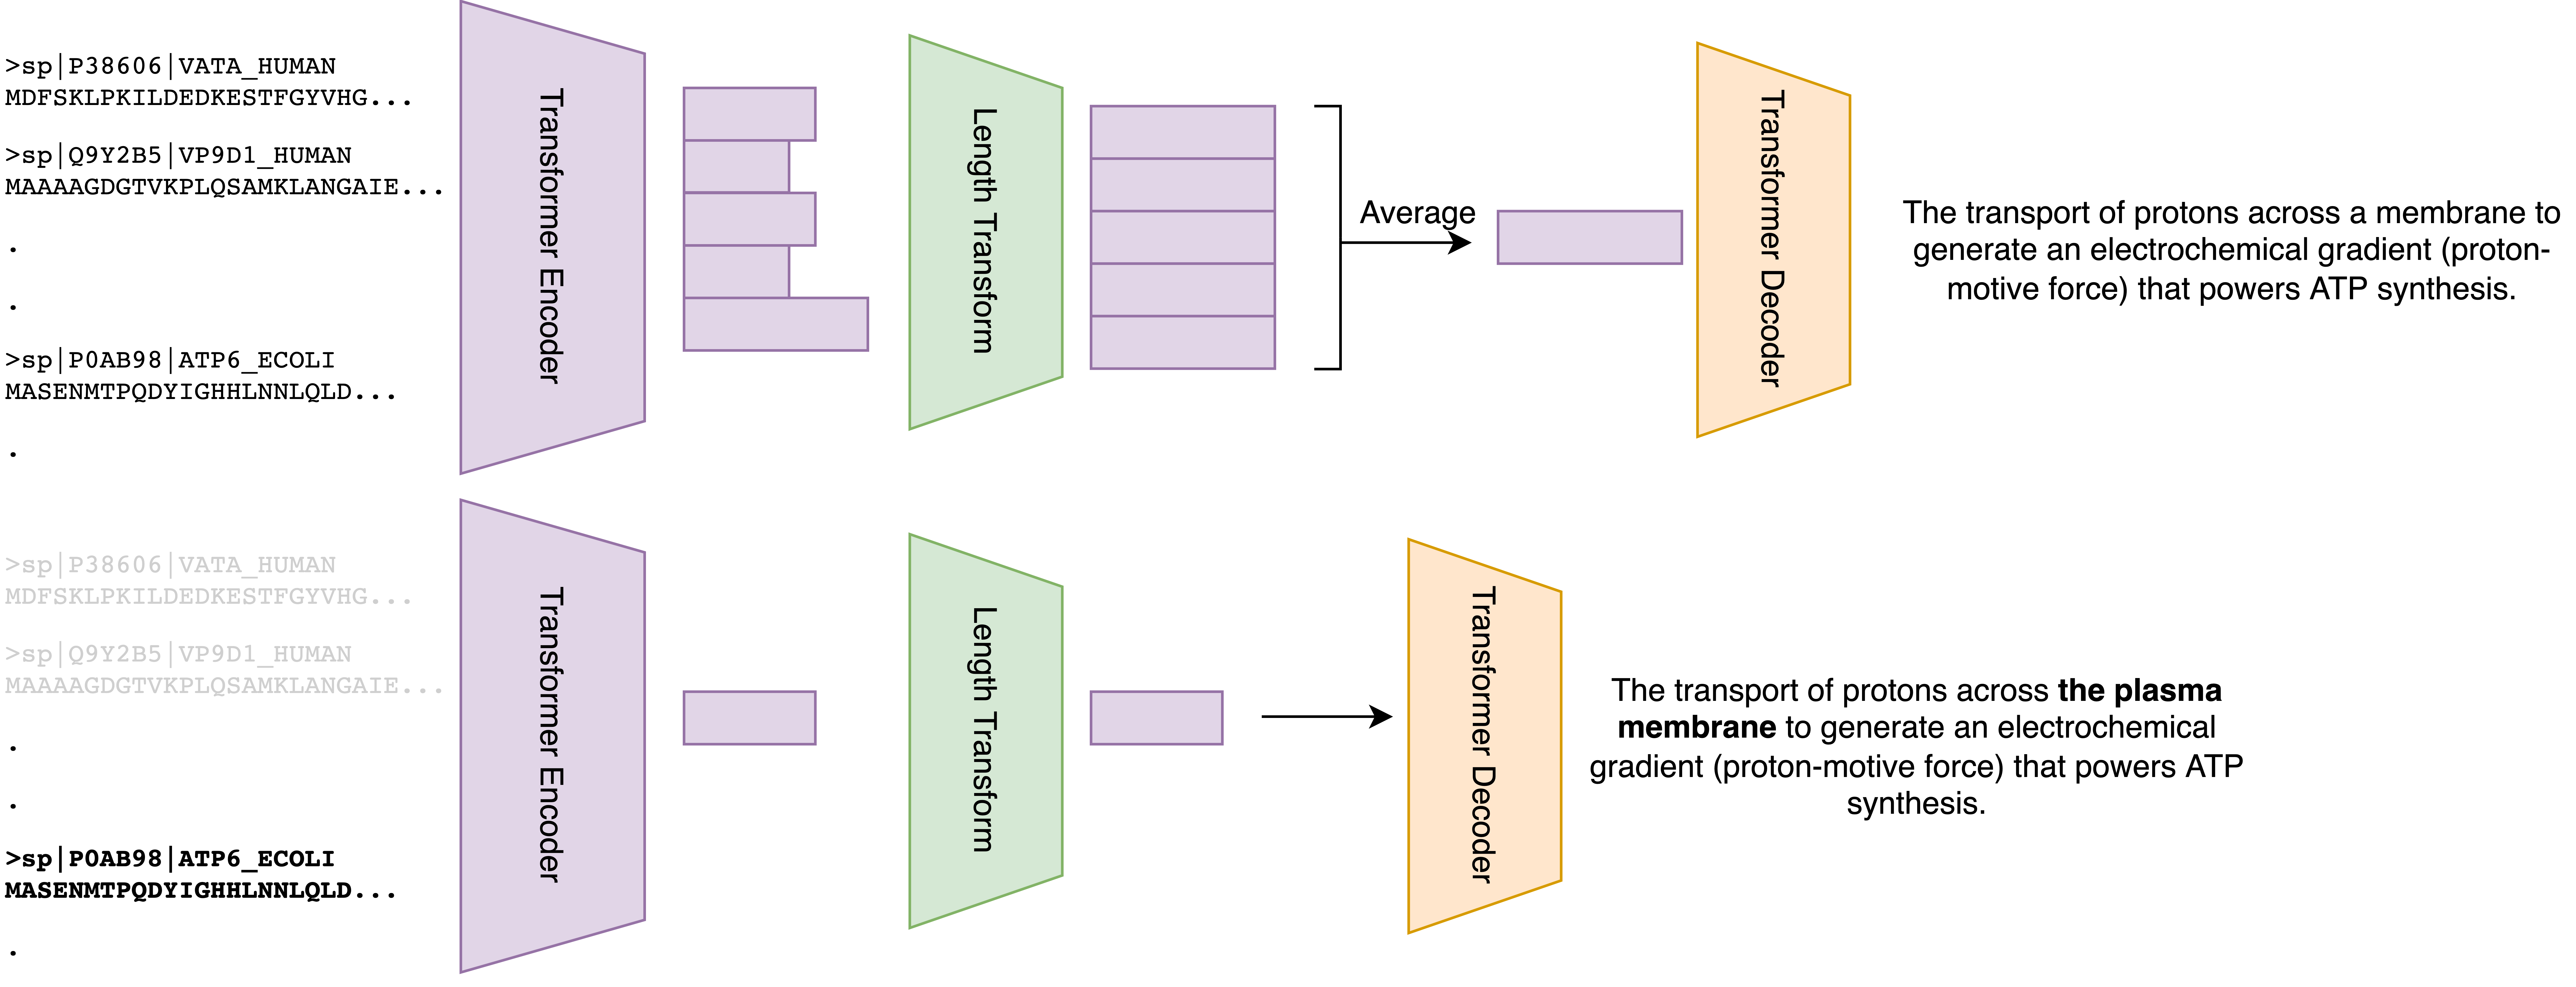
\includegraphics[width=0.9\linewidth]{prot2go.png}
    \caption{Transformer encoder-decoder model. Estimates $P(d|S)$ where S is a set of protein sequences and d is a given description.}
    \label{overview}
\end{figure}

\end{frame}

\begin{frame}
\frametitle{Key aspects of method}
\begin{enumerate}
    \item{Input: Protein sets to describe, invariant to order}\pause
%We begin describing our method with the way we construct our input.
        %We use sets of protein sequences, invariant to ordering, as input to the model giving a description. In this way, we are making the problem more general: our task is to describe the function of a set of any number of proteins. This matches the manual process of characterizing new functions. Biologists describe and categorize functions which are abstractions of the common behavior of groups of proteins in nature, so we want our model to be able to perform this abstraction given any set of proteins.
    \item{Autoregressive generation of descriptions}\pause
    \item{Evaluation}\pause
        \begin{itemize}
            \item{Description Generation: difficult to evaluate}\pause
            \item{Scoring descriptions of unseen categories (``zero-shot" classification)}\pause
            %Fundamentally, our model assigns probabilities to pairs of protein sets and descriptions. In order to evaluate the method, we use the zero-shot classification setting, where we wish to classify proteins into unseen categories. We develop three metrics in the Evaluation section to evaluate the distribution learned by the model in this classification setting.

        \end{itemize}
%Another contribution we make in proposing this method is to generate protein function descriptions in natural language. This allows for the characterization of proteins in a compositional way, with a grammar such that all protein sets can be described with the model, not just those with particular sets of terms the scientific community has manually assigned with the Gene Ontology.
    %\item{Implementation}\pause
    %    \begin{itemize}
    %    \item{Transformer encoder-decoder model}\pause
    %We use a transformer encoder-decoder model \cite{vaswani2017attention} with a length transform \cite{shu2020latent} to handle differing sequence lengths in order to average sequence features from the encoder.
        %\item{Length transform}\pause
        %The model takes sequences of varying length. The sequence features as they are produced by the model are not able to be pooled without losing information.
        %\item{Generation using beam search}
            % Generation of descriptions is a search problem through the set of all possible output token sequences, where the goal is to find the sequence with the largest probability. Generation given an autoregressive model is a highly studied problem in the natural language processing literature. We use beam search in the current implementation in order to find reasonable generated descriptions. Evaluation of these descriptions is an unsolved problem; currently, manual inspection by expert human evaluators is the best method we have.
        %\end{itemize}
    \end{enumerate}
\end{frame}

\begin{frame}
    \frametitle{How do you evaluate this model?}
    \begin{itemize}
        \item Evaluating \textit{generated} descriptions can really only be done manually. \pause
            \begin{itemize}
                \item This is not a solved problem in natural language processing.\pause
                \item Most work relies on manual ranking of generated text samples in terms of their similarity to a gold standard.\pause
            \end{itemize}
        \item We can, however, evaluate the scoring that the model assigns to pairs of sequence sets and their known descriptions.
    \end{itemize}
\end{frame}

\begin{frame}
\frametitle{Evaluation metrics}
Three things that we care about for generated descriptions:\pause
\begin{enumerate}
    \item Correctness: We want accurate descriptions about the protein set's function to be ranked higher than inaccurate ones.\pause
        \begin{itemize}
            \item Average number of times a correct description outranks an incorrect one\pause
        \end{itemize}
    \item Specificity: Among correct descriptions, we want descriptions that are more specific to be ranked higher than more general ones.\pause
        \begin{itemize}
            \item Average number of times a correct child term outranks its parent term(s)\pause
        \end{itemize}
    \item Robustness: For two sets of proteins that have the same common functions among each set, we want the correct descriptions' rankings to be the same for both sets.\pause
        \begin{itemize}
            \item Average Spearman's rank correlation of the sequence sets' correct terms\pause
        \end{itemize}

\end{enumerate}
\end{frame}

%\begin{frame}
%    \frametitle{Attribute 1: Annotation correctness.}
%        Descriptions of GO terms that annotate the entire sequence set should be scored higher than terms that do not.
%\end{frame}
%
%\begin{frame}
%    \frametitle{Attribute 1: Annotation correctness.}
%
%            Let $D_{S}$ be the set of GO term descriptions associated with sequence set S.\pause
%
%            \[P(d \in D_{S} | S) > P(d \notin D_{S} | S)\]\pause
%
%                We can calculate the average number of times a correct description outranks an incorrect one:
%        \[\frac{1}{|D_{S}|*|D_{S}^{c}|}\sum_{d_i \in D_{S}, d_j \notin D_{S}} \mathds{1}(P(d_i | S) > P(d_j | S))\]
%        where $D_{S}^{c}$ is the complement of $D_{S}$ and $\mathds{1}$ is the indicator function.
%
%\end{frame}
%
%\begin{frame}
%        \frametitle{Attribute 2: Specificity preference.}
%
%        Among correct terms, the model should score child terms higher than their parent terms.
%\end{frame}
%\begin{frame}
%        \frametitle{Attribute 2: Specificity preference.}
%
%Let $A(d)$ denote the description of a direct parent of the GO term described by $d$.\pause
%        We want:
%        \[P(d \in D_{S}| S) > P(A(d) \in D_{S}| S)\]\pause
%
%        We can calculate the average number of times a correct child term outranks its parent term(s):
%        \[\frac{1}{|D_{S}|}\sum_{d_i \in D_{S}} \mathds{1}(P(d_i | S) > P(A(d_i) | S))\]
%
%\end{frame}
%\begin{frame}
%    \frametitle{Attribute 3: Annotation robustness.}
%
%        Any pair of sequence sets that have the same GO descriptions in common should produce scores with the same rankings for those GO descriptions.
%\end{frame}
%
%\begin{frame}
%    \frametitle{Attribute 3: Annotation robustness.}
%        Let $S_i$ and $S_j$ be different sequence sets such that $D_{S_i} = D_{S_j}$, and let $R(X)$ be a ranking function that gives the rankings of probabilities in $X$.\pause
%
%        \[R_{d}(P(d \in D_{S_i} | S_i)) = R_{d}(P(d \in D_{S_i} | S_j))\]\pause
%
%        We can calculate the average Spearman's rank correlation of the rankings for all sequence sets' correct descriptions.\pause
%Let $R_{S_i} = R(P(D_{S_i} | S_i))$:
%
%        \[\frac{1}{N*(N-1)}\sum_{S_i, S_j} \frac{\textnormal{cov}(R_{S_i}, R_{S_j})}{\sigma_{R_{S_i}}\sigma_{R_{S_j}}}\]
%
%        where $N$ is the total number of sequence sets that have the exact set of GO descriptions $D_{S_i}$.
%In reality, this number may be too large to actually sum (especially if $|D_{S_i}|$ is small), so we approximate this measure by subsampling $n < N$ sequence sets to average over instead.
%The sum is only calculated over non-identical pairs of sequence sets.

%\end{frame}

\begin{frame}
    \frametitle{Data}
    \begin{itemize}
        \item Uniprot-KB Swiss-Prot (manually annotated and reviewed), 566,996 proteins total
        \begin{enumerate}
            \item Maximum number of proteins per GO term: 1280
            \item Minmum number of proteins per GO term: 32
            \item Total number of proteins in training set: 316k
            \item Total number of proteins in validation set: 180k
            \item Total number of GO terms in training set: 9053
            \item Total number of GO terms in validation set: 2264
        \end{enumerate}
    \end{itemize}
\end{frame}

\begin{frame}
\frametitle{Results}

\begin{table}
	\caption{Model Validation Set Performances}
	\centering
    \begin{tabular}{p{0.2\textwidth}|p{0.35\textwidth}|p{0.35\textwidth}}
		\toprule
        Metric & Model scores & Term-normalized model scores\\
		\midrule
        Correctness & 0.57 & 0.83\\
        Specificity & 0.52 & 0.58\\
        Robustness & 0.84 & 0.44\\
		\bottomrule
	\end{tabular}
	\label{tab:table}
\end{table}
\end{frame}

\begin{frame}
\frametitle{Description generation examples}
    \begin{itemize}
        \item Taking a Gene Ontology term that was not included in training\pause
        \item Sampling the proteins annotated with that term\pause
        \item Use these proteins as input to the model\pause
        \item Use beam search over token probabilities to generate tokens sequentially
    \end{itemize}
\end{frame}

\begin{frame}
\frametitle{Validation set generation examples}
GO:0032099: negative regulation of appetite

Actual description:

any process that reduces appetite .

Prediction:

any process that results in a change in state or activity of an organism ( in terms of a result of a leptin stimulus .
\end{frame}

\begin{frame}
\frametitle{Validation set generation examples}
GO:0003725: double-stranded RNA binding

Actual description:

binding to double-stranded rna .

Prediction:

any process that activates or increases the rate or extent of rrna molecule .
\end{frame}

\begin{frame}
\frametitle{Validation set generation examples}
GO:0035434: copper ion transmembrane transport

Actual description:

the directed movement of copper cation across a membrane .

Prediction:

the increase in size ( protons .
\end{frame}

\begin{frame}
\frametitle{Validation set generation examples}
GO:0046992: oxidoreductase activity, acting on X-H and Y-H to form an X-Y bond

Actual description:

catalysis of an oxidation-reduction ( redox ) reaction in which x-h and y-h form x-y .

Prediction:

the formation of methane , the formula ch4 .
\end{frame}

\begin{frame}
\frametitle{Validation set generation examples}
GO:0042023: DNA endoreduplication

Actual description:

regulated re-replication of dna within a single cell cycle , resulting in an increased cell ploidy . an example of this process occurs in the synthesis of drosophila salivary gland cell polytene chromosomes .

Prediction:

any process that modulates the frequency , rate or extent of chromatin organization .
\end{frame}

%\begin{frame}
    %\frametitle{Current experiments to do}
    %\begin{itemize}
        %\item Remove restriction of training/testing on functions with 32 to 1280 examples
        %\item Architecture search
        %\item Use byte-pair encoding instead of word-based encoding
        %\item Add label smoothing
        %\item Add oversmoothing regularization \footfullcite{Kulikov2021Oversmoothing}
        %\item Train on TREMBL annotations (more than 100 million proteins with some GO annotation, unreviewed)
    %\end{itemize}
%\end{frame}


\begin{frame}
\frametitle{Future human-assisted evaluation of function discovery}
%As our scoring metrics for evaluation are automated, they can be used for optimizing the architecture and other hyperparameters of the model (either manually or with some search method).
%However, in the case of actual use on proteins that are not very well studied, it can be difficult to know whether a given description is accurate.
\begin{itemize}
    \item Human-assisted evaluation will be needed for the descriptions generated for a given set of novel proteins.\pause
    \item One possible way of obtaining human feedback would be to ask an expert Gene Ontology curator to choose between two descriptions for a given sequence set that is generated from a trained model.\pause
        \begin{itemize}
            \item This would be expensive, as the task needs to be done by an expert.\pause
        \end{itemize}
    \item This feedback could be used to fine-tune the model to produce more accurate, fluid or generally desirable descriptions of proteins, as has been done for document summarization models \footfullcite{learningToSummarize, finetuningWithHuman}.
    %\item Richer information, such as ranking the similarities to an existing GO term, or suggesting changes to particular portions of the description, could be used to increase performance even with a small number of examples with human feedback.
\end{itemize}
\end{frame}

\begin{frame}
\begin{columns}
    \column{0.3\textwidth}
    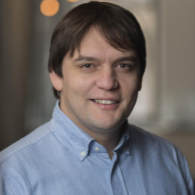
\includegraphics[width=0.8\columnwidth]{vlad.png}
    Vladimir Gligorijevic
    \column{0.3\textwidth}
    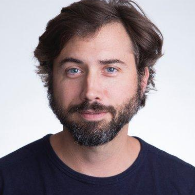
\includegraphics[width=0.8\columnwidth]{rich.png}
    Richard Bonneau
    \column{0.3\textwidth}
    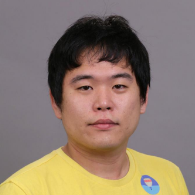
\includegraphics[width=0.8\columnwidth]{kyunghyun.png}
    Kyunghyun Cho
\end{columns}
\vfill
\begin{columns}
    \column{\textwidth}
    \centering Contact me at meetbarot@nyu.edu
\end{columns}

\end{frame}

\end{document}
